\section{Klassendiagram}
\subsection{Overzicht}
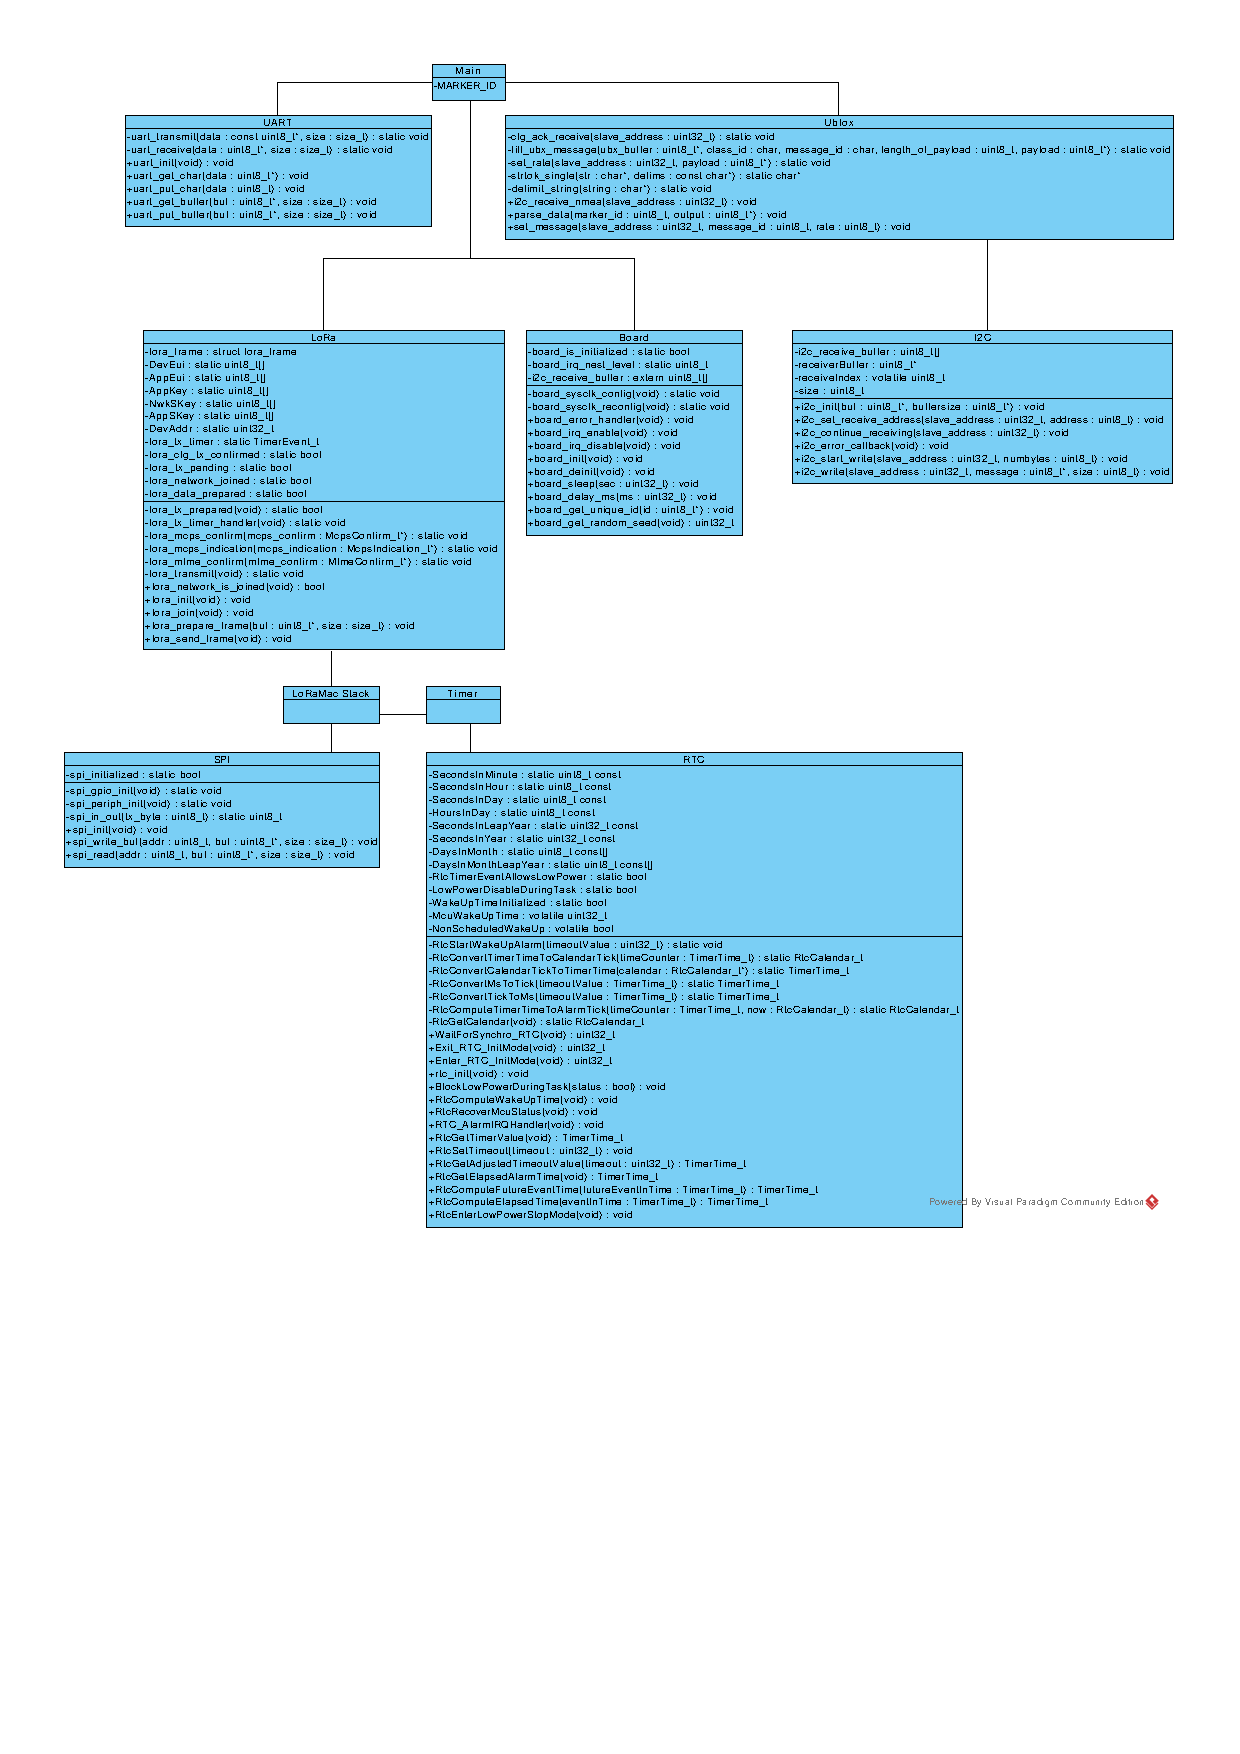
\includegraphics[width=0.9\textwidth]{technical/class_diagram.pdf}

\subsection{Eigen code}
\subsubsection{Main}
Dit is het entry point van de C code. Deze file bevat alleen de code die van belang
is voor de user, dat betekent dat de code zo simpel mogelijk is gehouden.

De user applicatie kijkt of de Smart Marker met een LoRaWAN netwerk verbonden is
en, zo ja, verstuurt dan de gemeten GPS-data over het netwerk. Wanneer er nog
geen verbinding is blijft hij proberen om connectie te maken.

\subsubsection{Board}
In dit interface staan de board ondersteunende functies (b.v. het uitschakelen van
interrupts) die door heel de programmatuur worden gebruikt.

De user applicatie zal niet werken als \texttt{board\_init()} niet als eerste
functie wordt aangeroepen.

\subsubsection{UART}
Deze driver wordt in de user applicatie doorgaans niet gebruikt, maar deze is
ontwikkeld om het debuggen makkelijker te maken.

\subsubsection{I2C}
Het I2C interface is ontwikkeld om de GPS-module uit te kunnen lezen. De inkomende
data wordt in een buffer opgeslagen, die in het \texttt{Ublox} interface wordt
uitgelezen.

\subsubsection{SPI}
Het SPI interface is geschreven om de LoRa radio registers te programmeren. Het
is ook te gebruiken om de GPS-module uit te lezen, echter is dat niet gebruikt in
deze applicatie.

\subsubsection{RTC}
De Real-Time Clock wordt gebruikt in het \texttt{Timer} interface, wat door Semtech
is ontwikkeld. De RTC stelt een interrupt in, zodat het board wakker gemaakt kan
worden op de gewenste datum of het gewenste tijdstip.

\subsubsection{LoRa}
Dit interface dient als laag tussen de user applicatie en de \texttt{LoRaMac} ofwel
de LoRaWAN netwerk stack. Het is geschreven om de werking en instellingen van LoRaWAN
te abstraheren voor de gebruiker. Zo is het makkelijker om een andere user applicatie
te schrijven.

\subsubsection{Ublox}
Het Ublox interface is geschreven specifiek voor de GPS-module die gebruikt is
tijdens dit project. Het staat de gebruiker toe om instellingen te veranderen in
de module, zodat b.v. het krijgen van een GPS-fix minder lang duurt, of om de
frequentie van berichten in te stellen.

\subsection{Gebruikte code}
Omdat het draait om de code die de studenten hebben geproduceerd, is gebruikte
code zoveel mogelijk buiten het klassendiagram gehouden.

\subsubsection{LoRaMac van Semtech}
Semtech, de producent van de LoRa chips, heeft in samenwerking met wat kleinere
bedrijven een implementatie gemaakt die overeenkomen met de LoRaWAN specificaties.
Dit project, genaamd LoRaMac, is gebruikt als basis voor de Smart Marker LoRa
implementatie.

Deze code staat in de directory: \texttt{code/smart\_marker/lora}.

\subsubsection{STM32L0xx CMSIS / low-layer drivers}
STMicroelectronics, de producent van het development board waarmee gewerkt is,
heeft een aantal board ondersteunende soft-/firmware pakketten die het makkelijker
maken om te ontwikkelen met de hardware.

Deze code staan in de directories:
\begin{itemize}
    \item \texttt{code/smart\_marker/bsp/cmsis}
    \item \texttt{code/smart\_marker/bsp/stm32l0xx\_hal}
\end{itemize}